% !TeX spellcheck = en_US
\section{Empirical Analysis}\label{sec:Analysis}

 In this section, we present our empirical results, starting with a descriptive overview of the measured \textsf{keyATM} topics between 2019 and 2023. Next, we introduce our polarity score, which measures media reports on rising or falling inflation rates based on word embeddings. By integrating our polarity analysis with the results from the \textsf{keyATM}, we derive our final narrative indices. Utilizing these indices, we conduct multivariate Granger causality tests to assess the predictive power of our measured narratives. By disaggregating household expectations, we are able to identify differences based on a range of socio-economic factors. Finally, we employ local projections to study the effect of narrative diffusion on the macroeconomy.

\subsection{Narrative Topics}\label{subsec:atmtopics}

We begin by examining the interpretability of the resulting topics, following the procedure recommended by \citet{Eshima.2023}, and provide an overview of the topic-word distribution. In other words, we highlight terms with high probabilities of topic selection. These terms are visualized in figure \ref{fig:wordclouds} as wordclouds for each of the considered topics. The wordclouds highlight the topics' consistency with the underlying narrative concept. Moreover, multiple pre-selected keywords are present for the vast majority of topics. The presence of multiple keywords and topic-consistent terms suggests a successful measurement of the respective concepts. To illustrate: terms like ``unemployment'', ``work'', and ``growth'' are close to the labor shortage narrative, while ``share'', ``revenue'', and ``rise'' are closely related to the profit narrative. An exception is the pent-up demand topic, for which none of the top 20 words includes a pre-selected keyword. Despite this, we observe a predominant use of words associated with the overarching narrative of economic recovery, featuring words like ``rise'', ``growth'', and ``increase''.

Following the discussion on consistency, we consider the development of topic proportions over time. As figure \ref{fig:narr_all} illustrates, there are some major changes present over time. The pandemic topic surge stands out overall. It is marked by a sudden increase that is sustained with elevated shares until the conclusion of 2022. The strong increase in the war topic is also sudden, although of short duration. More generally, proportions start to shift in 2021, when inflation rates began to rise. Significant steady increases are observed for the demand shift, supply chain, energy, and profits topics. Among these, the most notable increases are reported for the supply chain and demand shift topics. Additionally, the government spending and labor shortage topics experience slight increases. However, the latter already starts declining in 2021. We observe more fluctuations for the pent-up demand topic. It is characterized by losses in early 2020 but recovers and gains importance, especially at the end of 2022.

\begin{figure}[H]
	\centering
	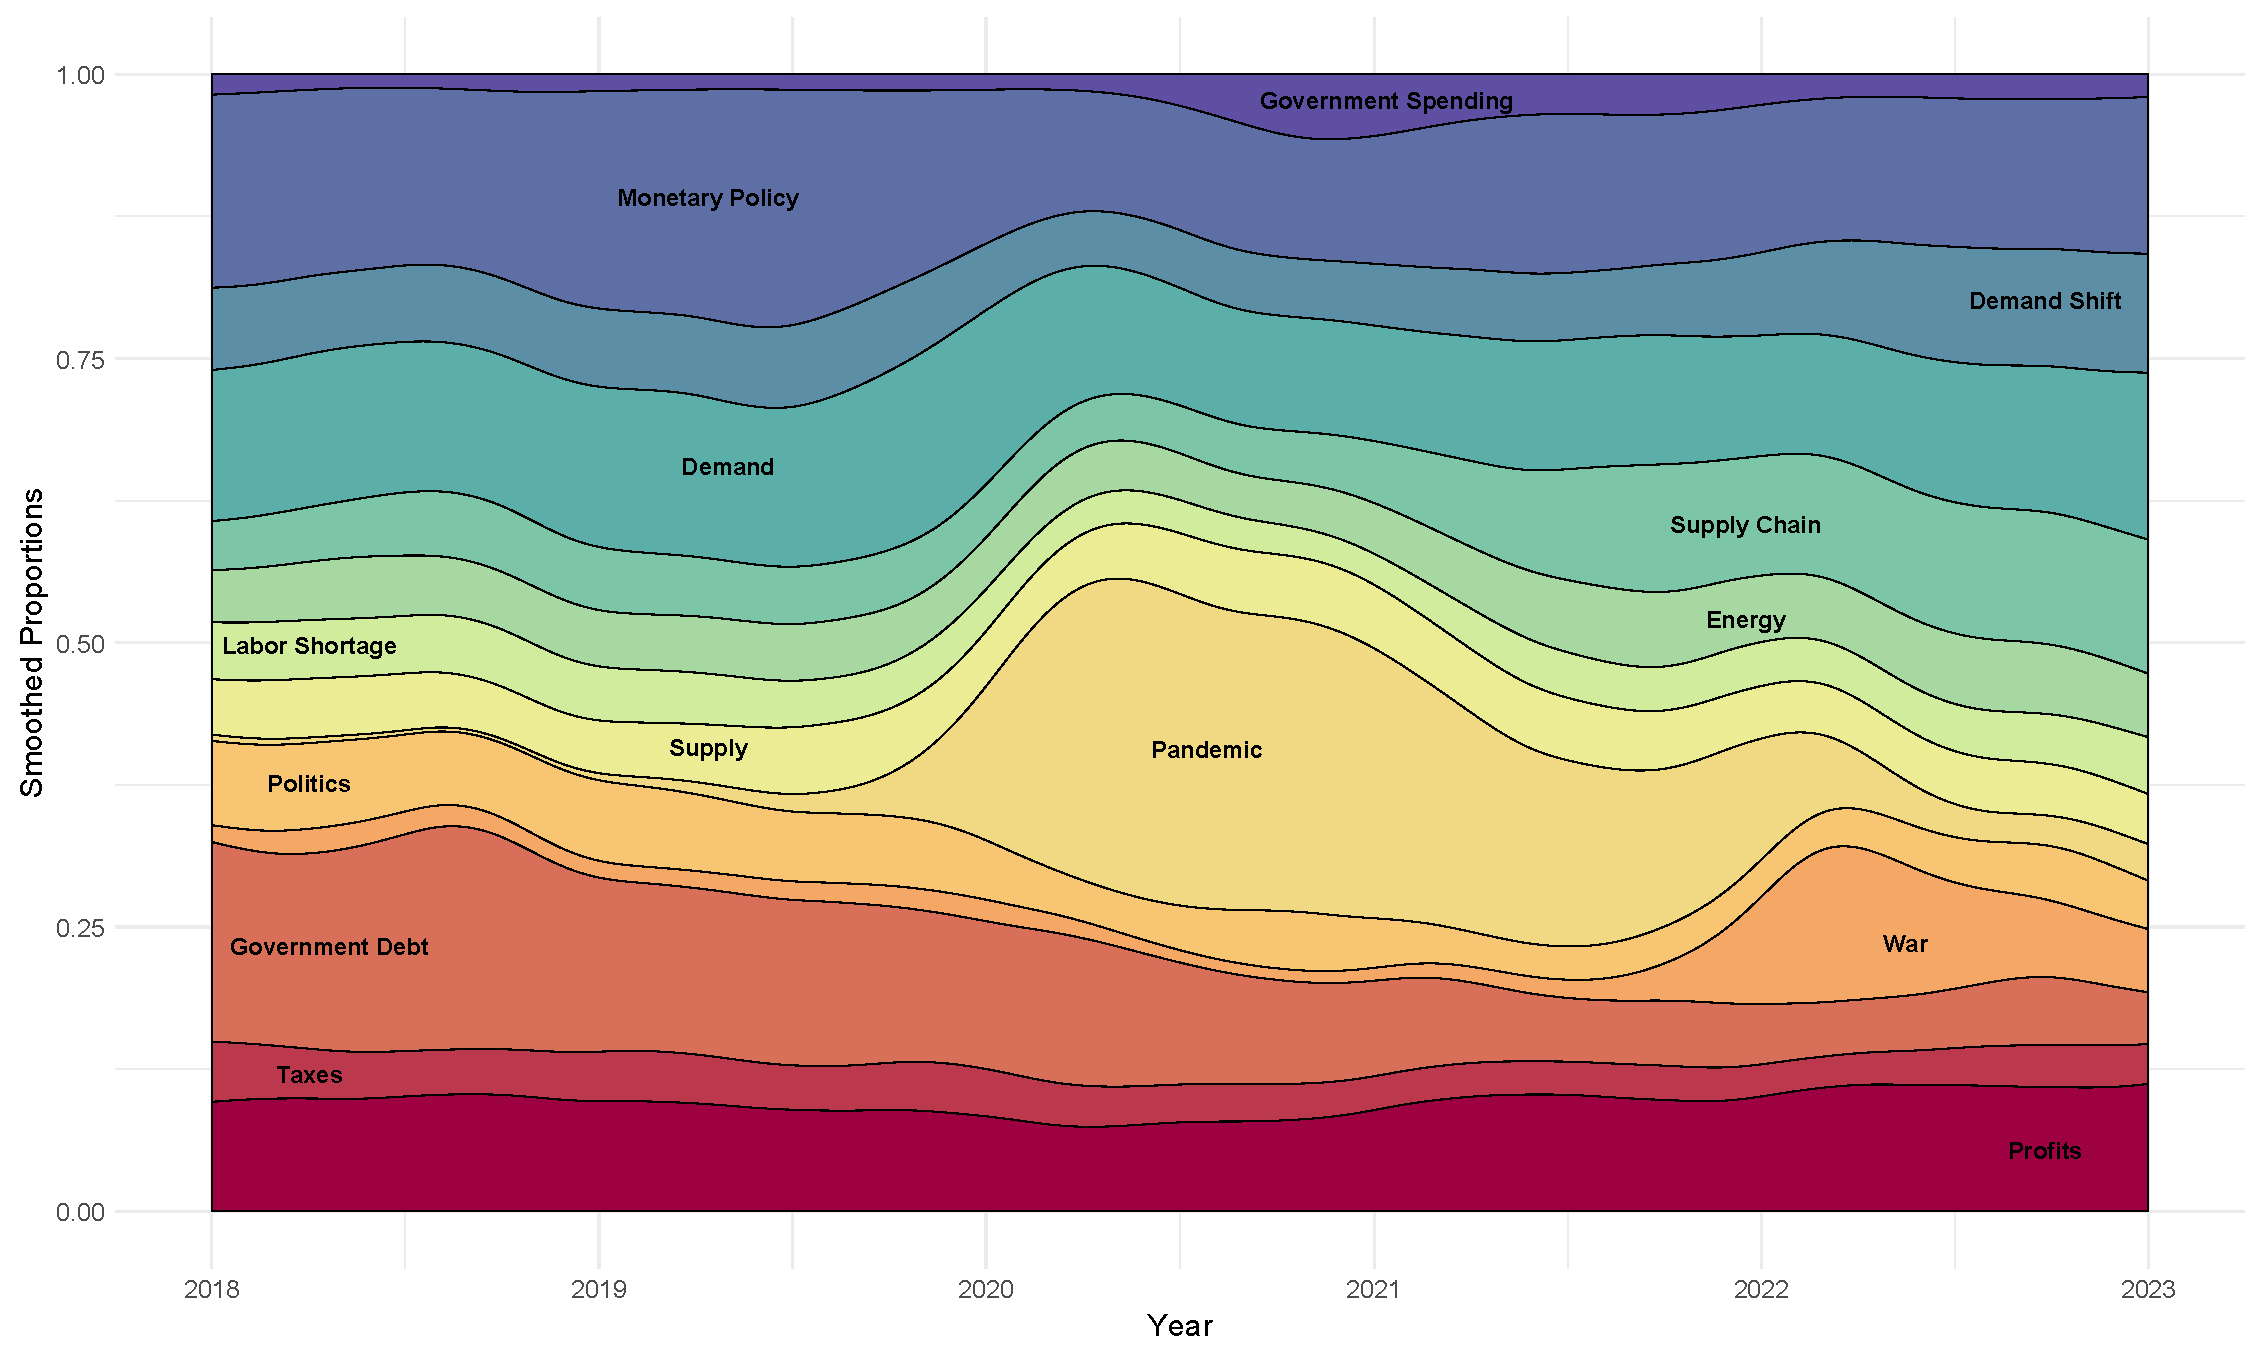
\includegraphics[width=0.65\linewidth, angle = 270]{figures/narratives_all.eps}
	\caption{Change of smoothed proportions}
	\label{fig:narr_all}
	\floatfoot{Note: The figure shows the development of the smoothed proportions. To calculate the relative proportions only the topics with pre-specified keywords were considered. To build this plot we employed the \textsf{geom\_stream()} function by \cite{Sjoberg.2021}. We organized the topics by following the code system provided by \cite{Andre.2023}.} 
\end{figure}

We observe a similar picture in the monetary policy topic. It also declines during the early phase of the pandemic, however, it shows recovery towards the end of the observation period. On the contrary, the debt topic shows a more steady decline. This topic is characterized by only occasional minor increases during the outbreak of the pandemic. The tax topics maintained relatively stable shares throughout the observation period, whereas the politics topic shows more fluctuations. It experiences an increase at the end of 2020, coinciding with the presidential election. Additionally, we observe a slight increase in relative importance towards the end of 2022.

To ensure robustness irrespective of the news structure, we provide a subsample comparison \textsf{keyATM} estimation that only includes Wall Street Journal (WSJ) articles, as illustrated in figure \ref{fig:comparision} in the Online Appendix. The WSJ corpus includes approximately 25,500 documents. While most topics exhibit similar trajectories, a few minor differences are observed. On the one hand, smaller volumes for the pandemic and supply chain topics are found in the WSJ corpus. However, a simultaneous trend is present. On the other hand, the politics topic shares are greater with the WSJ corpus. Overall, the topics in the WSJ corpus appear to react more strongly to singular events compared to the baseline corpus, which includes more financial and corporate sources.

\begin{figure}
	\begin{subfigure}{0.32\textwidth}
		\includegraphics[width=0.7\textwidth,angle=270]{figures/wordcloud7.eps}
		\caption{Government spending}
	\end{subfigure}
	\begin{subfigure}{0.32\textwidth}
		\includegraphics[width=0.7\textwidth,angle=270]{figures/wordcloud6.eps}
		\caption{Monetary policy}
	\end{subfigure}
	\begin{subfigure}{0.32\textwidth}
		\includegraphics[width=0.7\textwidth,angle=270]{figures/wordcloud8.eps}
		\caption{Pent-up demand}
	\end{subfigure}
	\begin{subfigure}{0.32\textwidth}
		\includegraphics[width=0.7\textwidth,angle=270]{figures/wordcloud9.eps}
		\caption{Demand shift}
	\end{subfigure}
	\begin{subfigure}{0.32\textwidth}
		\includegraphics[width=0.7\textwidth,angle=270]{figures/wordcloud5.eps}
		\caption{Supply chain}
	\end{subfigure}
	\begin{subfigure}{0.32\textwidth}
		\includegraphics[width=0.7\textwidth,angle=270]{figures/wordcloud4.eps}
		\caption{Labor shortage}
	\end{subfigure}
	\begin{subfigure}{0.32\textwidth}
		\includegraphics[width=0.7\textwidth,angle=270]{figures/wordcloud1.eps}
		\caption{Energy}
	\end{subfigure}	
	\begin{subfigure}{0.32\textwidth}
		\includegraphics[width=0.7\textwidth,angle=270]{figures/wordcloud3.eps}
		\caption{Pandemic}
	\end{subfigure}
	\begin{subfigure}{0.32\textwidth}
		\includegraphics[width=0.7\textwidth,angle=270]{figures/wordcloud2.eps}
		\caption{War}
	\end{subfigure}
	\begin{subfigure}{0.32\textwidth}
		\includegraphics[width=0.7\textwidth,angle=270]{figures/wordcloud11.eps}
		\caption{Politics}
	\end{subfigure}
	\begin{subfigure}{0.32\textwidth}
		\includegraphics[width=0.7\textwidth,angle=270]{figures/wordcloud12.eps}
		\caption{Debt}
	\end{subfigure}
	\begin{subfigure}{0.32\textwidth}
		\includegraphics[width=0.7\textwidth,angle=270]{figures/wordcloud13.eps}
		\caption{Taxes}
	\end{subfigure}
	
	\begin{subfigure}{0.32\textwidth}
		\includegraphics[width=0.7\textwidth,angle=270]{figures/wordcloud10.eps}
		\caption{Profits}
	\end{subfigure}

	\caption{Wordclouds of \textsf{keyATM} keyword topics}
	\label{fig:wordclouds}
\end{figure}
\newpage

  
  
 
\subsection{Polarity-adjusted Narrative Time Series}
So far, using a \textsf{keyATM} model enables us to measure reports on various causes of inflation. However, a key challenge lies in discerning the directions of these arguments, significantly impacting the subsequent econometric time series analysis. As detailed in \ref{subsec:methods}, we address this issue by employing \textsf{LSS} to identify whether a document is mainly about (expected) rising or falling inflation rates. \cite{Ellen.2022} previously highlighted this methodological challenge. However, by applying a simple dictionary method, their approach falls short ``[...] to identify the difference in tonality for specific narratives, for example, with respect to inflation, and not only the overall contribution'' \citep[1533]{Ellen.2022}. In contrast, our approach enhances this methodology by employing semantic scaling to create a case-specific dictionary that identifies the narrative components’ tonality. Subsequently, we construct an index for each narrative by multiplying the sentiment score of a document by the relative proportions of the \textsf{keyATM} topics in each document. This is concluded by aggregating our data on monthly-level, resulting in the final indices of the narratives.

\begin{figure}[H]
	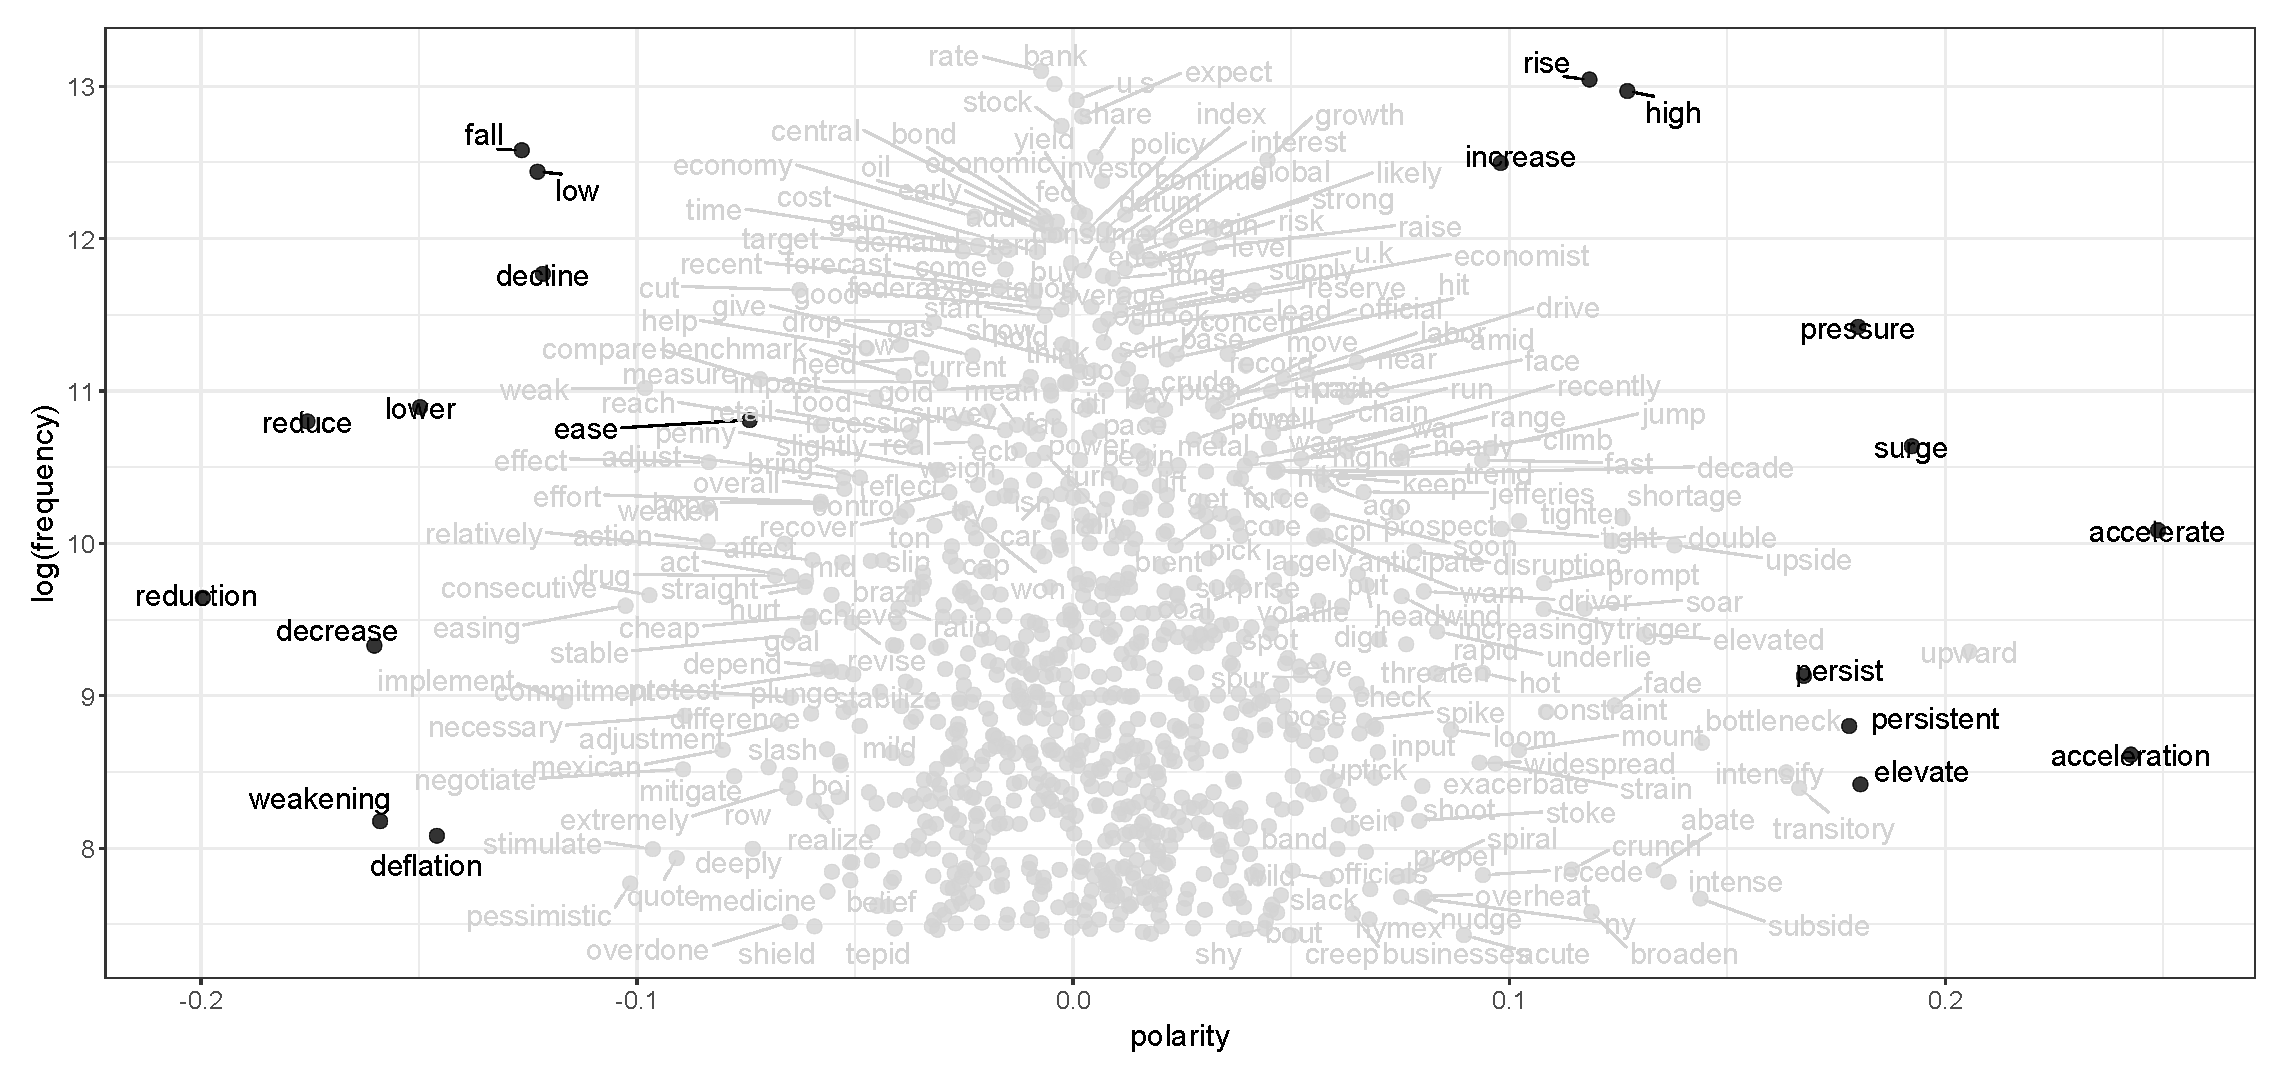
\includegraphics[width=1\textwidth]{figures/lss_words.eps}
	\caption{Polarity of words (seed words highlighted)}
	\label{fig:polarity}
	\floatfoot{Note: The figure shows the polarity scores for all statistically significant words around the target words ``infla*'' and ``price*''. To compute the polarity score, the semantic closeness towards pre-selected seed words are considered. To facilitate orientation, the utilized seed words are highlighted.} 
\end{figure}

 To evaluate the results of \textsf{LSS}, we plot the polarity scores constructed from our chosen seed words in figure \ref{fig:polarity}. The pre-selected seed words are highlighted in the figure. Those terms associated with falling inflation rates, such as ``deflation'', ``negative'', or ``downturn'' possess a negative polarity score. In contrast, terms like ‘intensify,’ ‘tight,’ or ‘shortage’ have a positive score. Additionally, the majority of words is located around the midpoint of the polarity score line. This is reasonable because most words are not implicitly associated with changing inflation rates. Examples, such as "affect," "likelihood," and "expect," share the characteristic of not being explicitly aligned with discussions about increasing or decreasing inflation rates. Thus, this observed neutrality can be interpreted as further validation for how accurate the estimation is. 
 
By weighting the polarity scores for each document, as described in \ref{subsec:methods}, we construct an aggregated polarity score at the document level. Figure \ref{fig:sentiment} shows the smoothed polarity score over time. As the plot demonstrates, the polarity score experiences strong fluctuations over the observation period. The figure shows a profound decline in the polarity score since the end of 2018. This trend corresponds with the realized CPI inflation, which began to decrease in mid 2018 and maintained low levels through October 2019. During this period, the US economy experiences a slowdown in growth. This is followed by a brief recovery of the inflation polarity, starting a the end of 2019. While the overall CPI inflation remained relatively low, an upward trend was still evident \footnote{For comparison: U.S. Bureau of Labor Statistics, Consumer Price Index for All Urban Consumers: All Items in U.S. City Average [CPIAUCSL], retrieved from FRED, Federal Reserve Bank of St. Louis; https://fred.stlouisfed.org/series/CPIAUCSL, February 21, 2024.}. Following the first lockdowns, we observe an increase in the polarity score starting in mid-2020. The score turns overall positive in 2021 and remains so until late 2022, peaking in late 2021.

\begin{figure}[H]
	\centering
	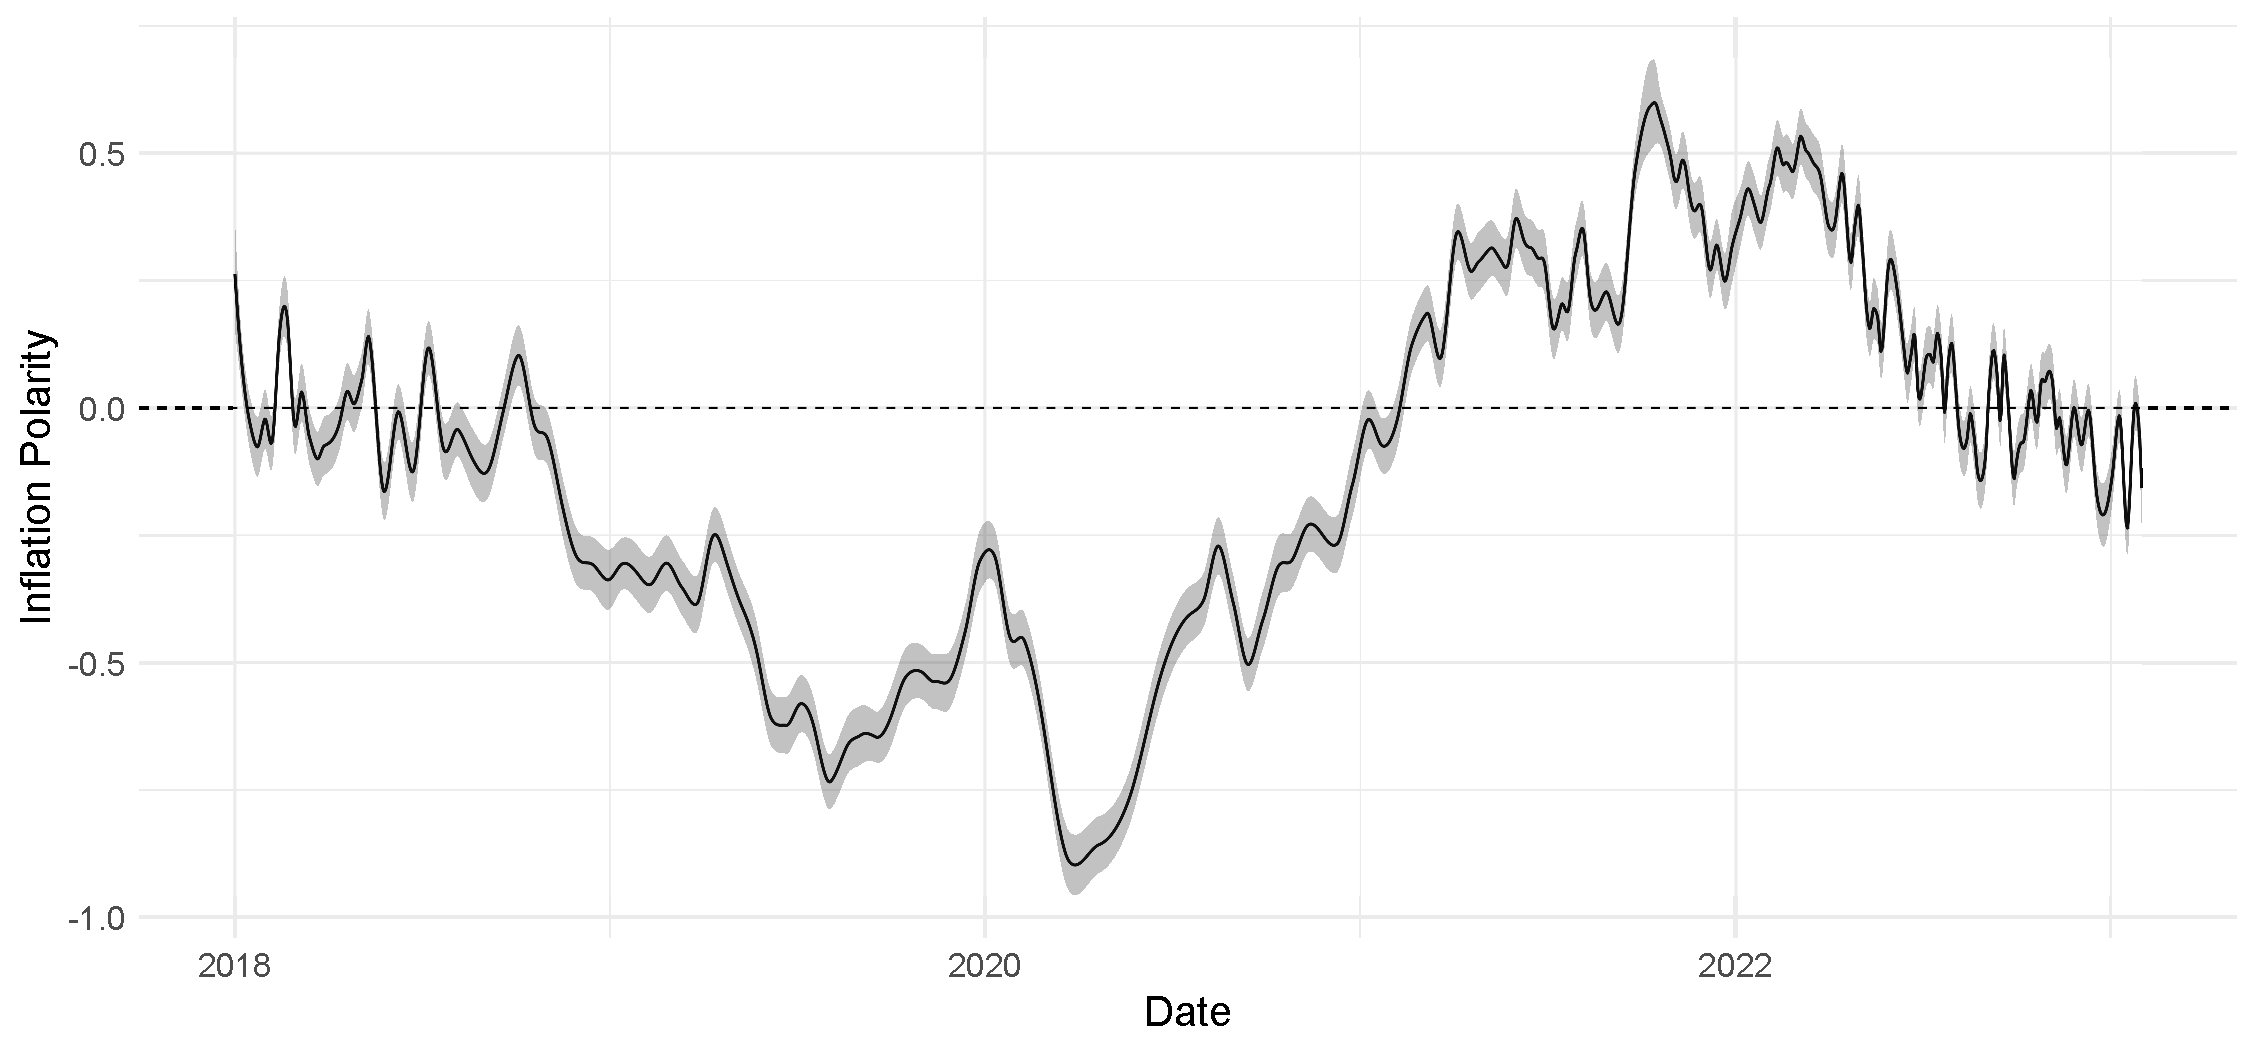
\includegraphics[width=0.95\linewidth]{figures/sentiment.eps}
	\caption{Change of polarity in corpus}
	\label{fig:sentiment}
		\floatfoot{Note: The figure shows the development of the aggregated polarity score computed by \textsf{LSS}. To ensure readability, the time series is smoothed by applying a local polynomial regression \citep{Watanabe.2023} with 95\% confidence intervals.} 
\end{figure}



Lastly, by combining our \textsf{keyATM} and \textsf{LSS} results, we construct the final narrative indices. We begin with the demand narratives, which are visualized in figure \ref{fig:sdemand}. As the figure illustrates, the demand inflation narratives are present during two considered periods: the non-inflationary (pre- and early pandemic) and the inflationary period (particularly since 2021). Until mid-2020, narratives highlighting monetary policy and pent-up demand factors are particularly prominent. The importance of the monetary policy narrative is exceptionally strong in mid-2019, meaning that a large number of reports about falling inflation rates were discussing aspects of monetary policy. This coincides with the previously discussed fall of the CPI rate under the inflation target. It also marks the first interest rate cut by the Fed in eleven years \citep{fed.2019}. In late 2021, the narrative reaches positive values and gains relative significance in the media coverage about rising inflation rates.
\begin{figure}[H]
	\begin{subfigure}[b]{0.95\textwidth}
		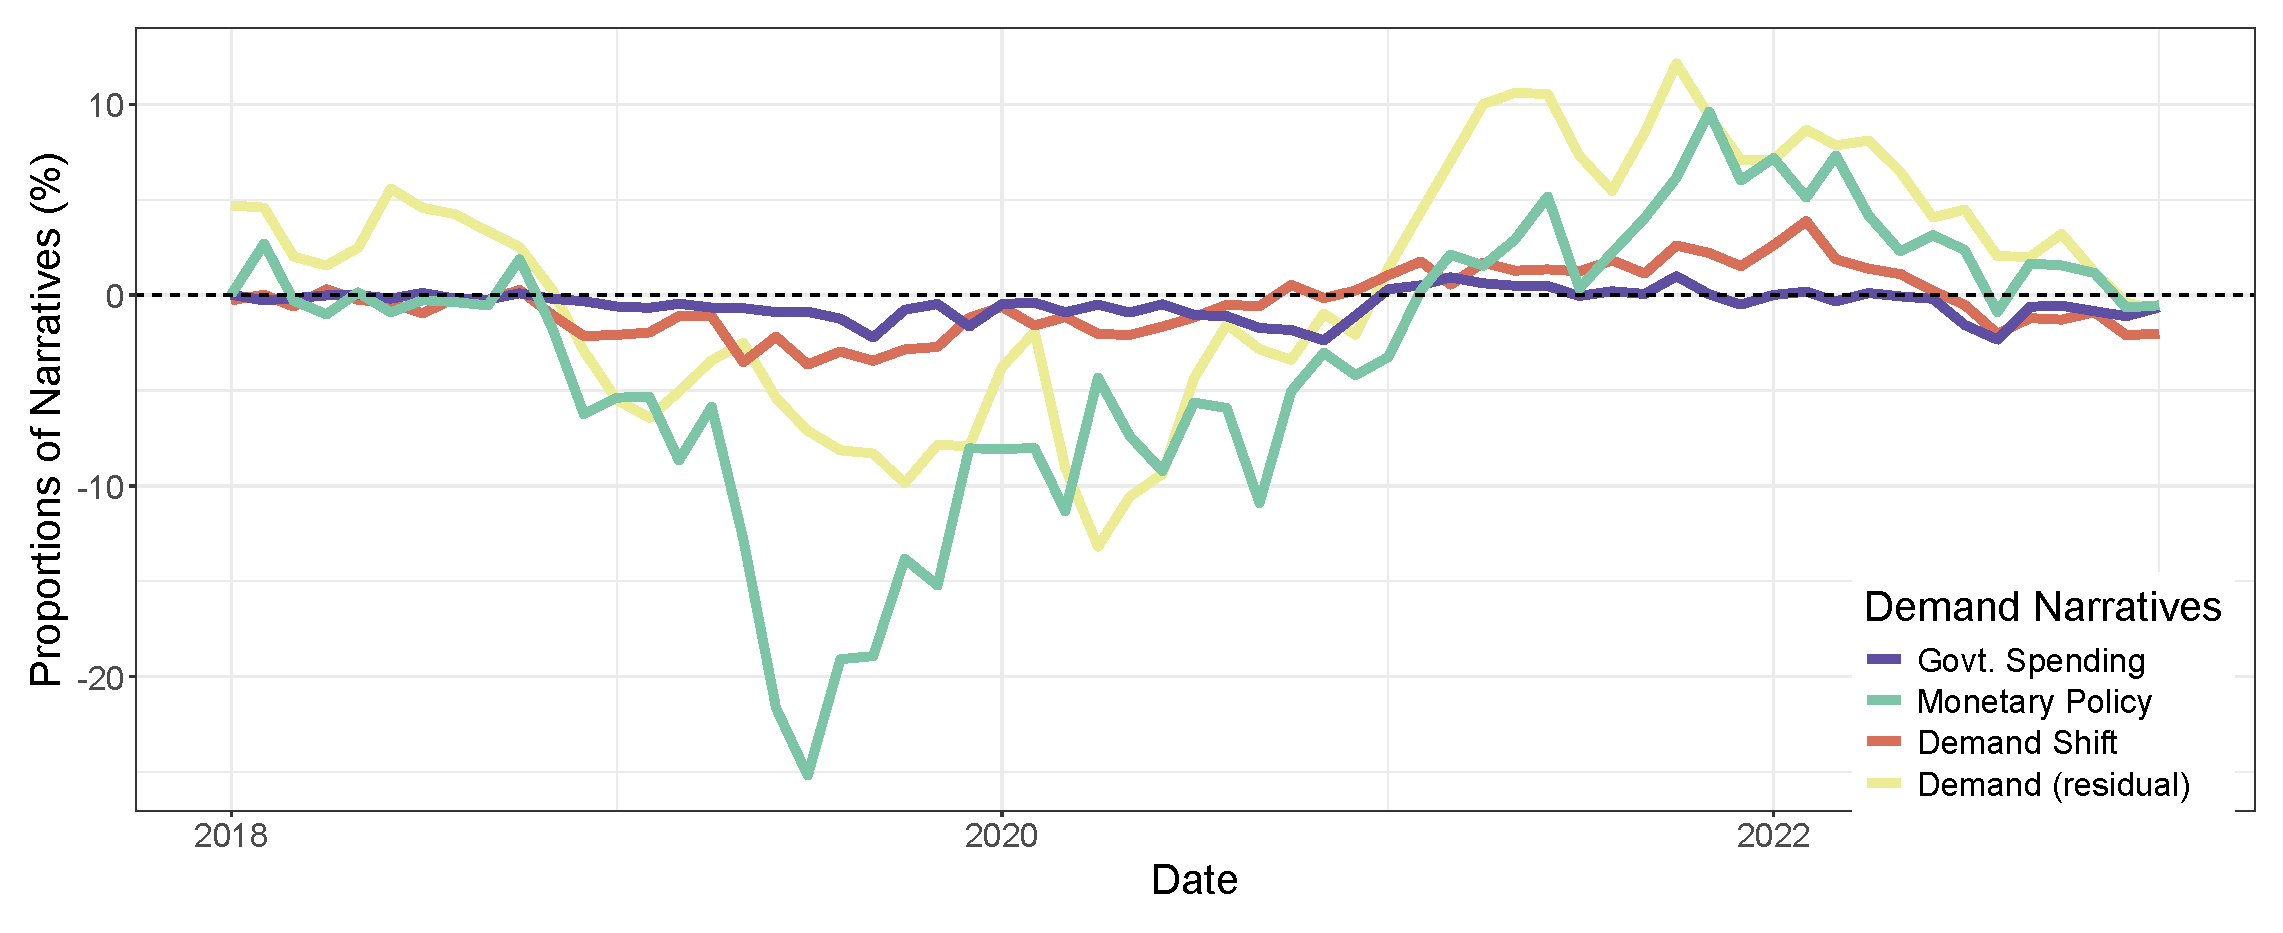
\includegraphics[width=\textwidth]{figures/plot_sdemand.eps}
		\caption{Indices of demand narratives}
		\label{fig:sdemand}
	\end{subfigure}
	\hfill
	\begin{subfigure}[b]{0.95\textwidth}
		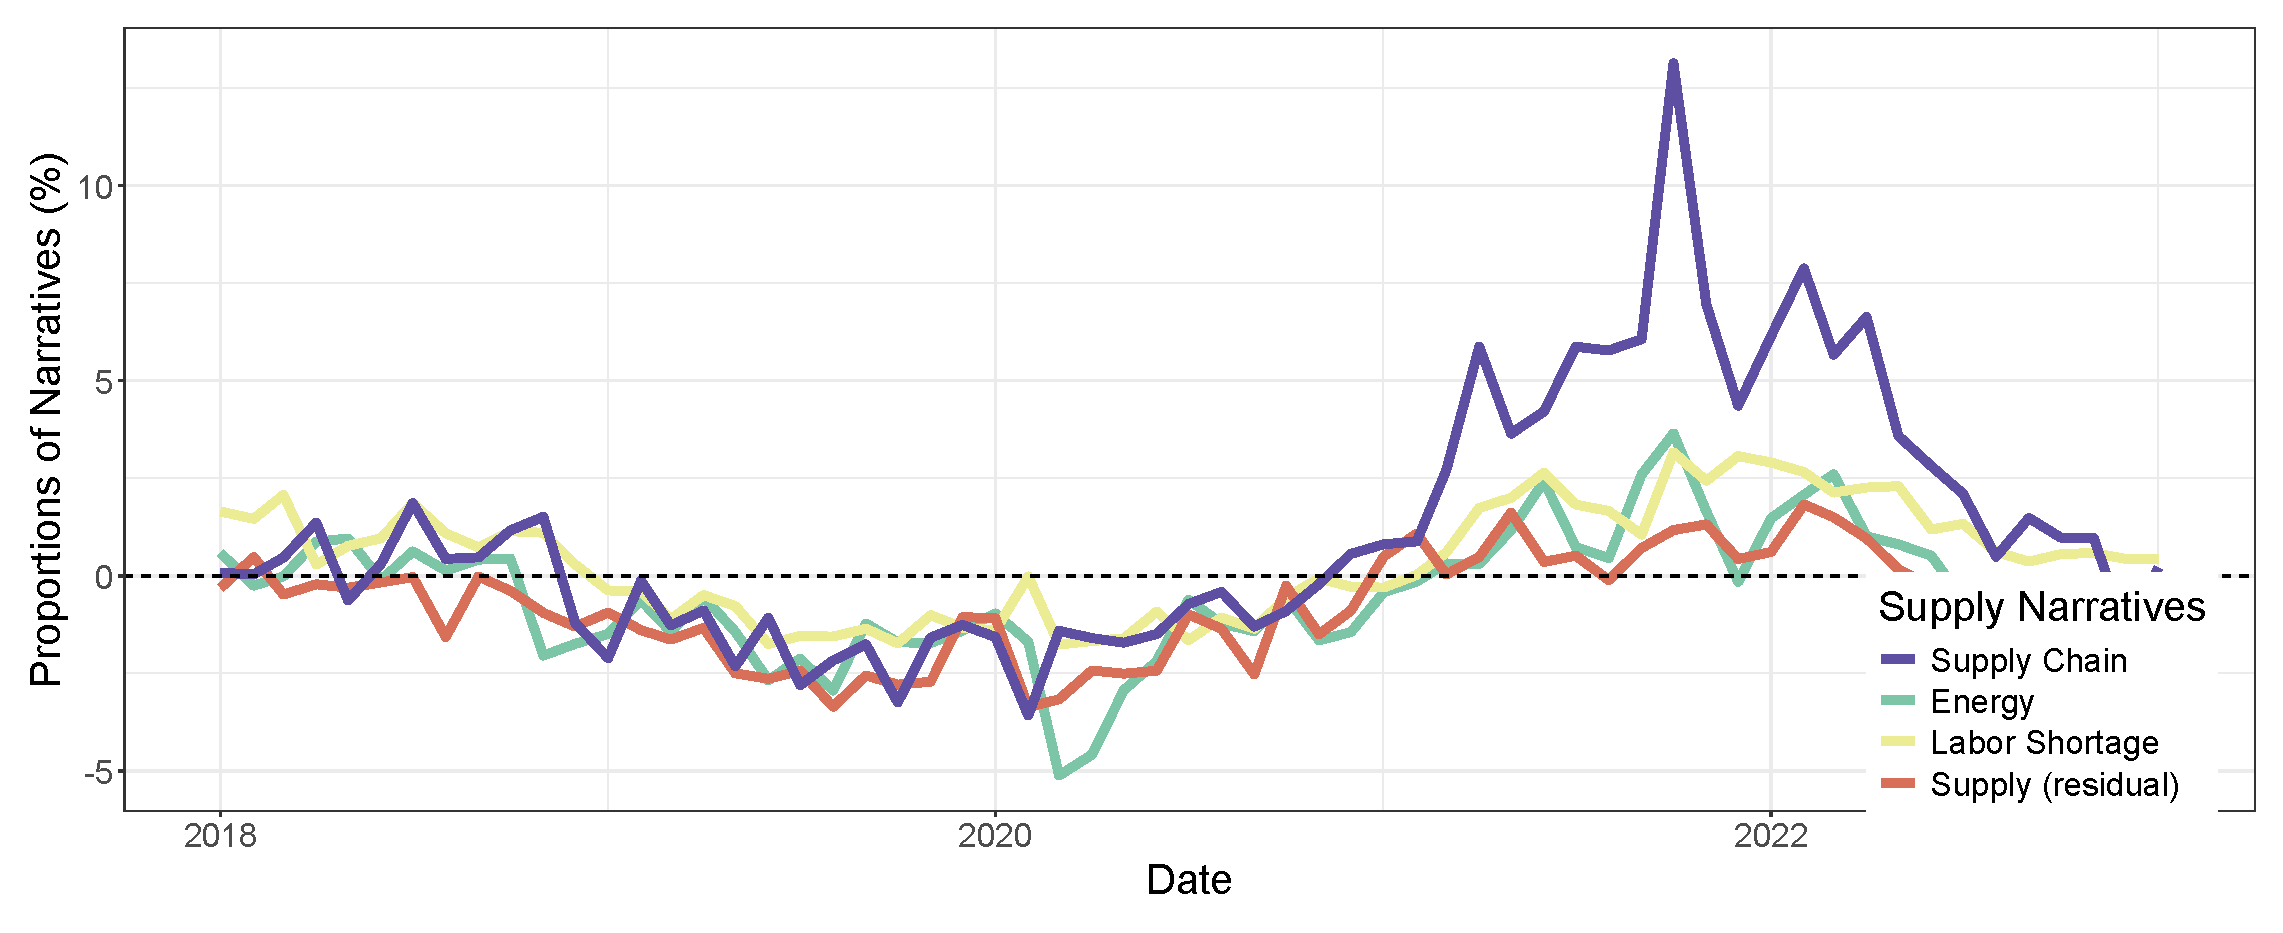
\includegraphics[width=\textwidth]{figures/plot_ssupply.eps}
		\caption{Indices of supply narratives}
		\label{fig:ssupply}
	\end{subfigure}
	\hfill
	\begin{subfigure}[b]{0.95\textwidth}
		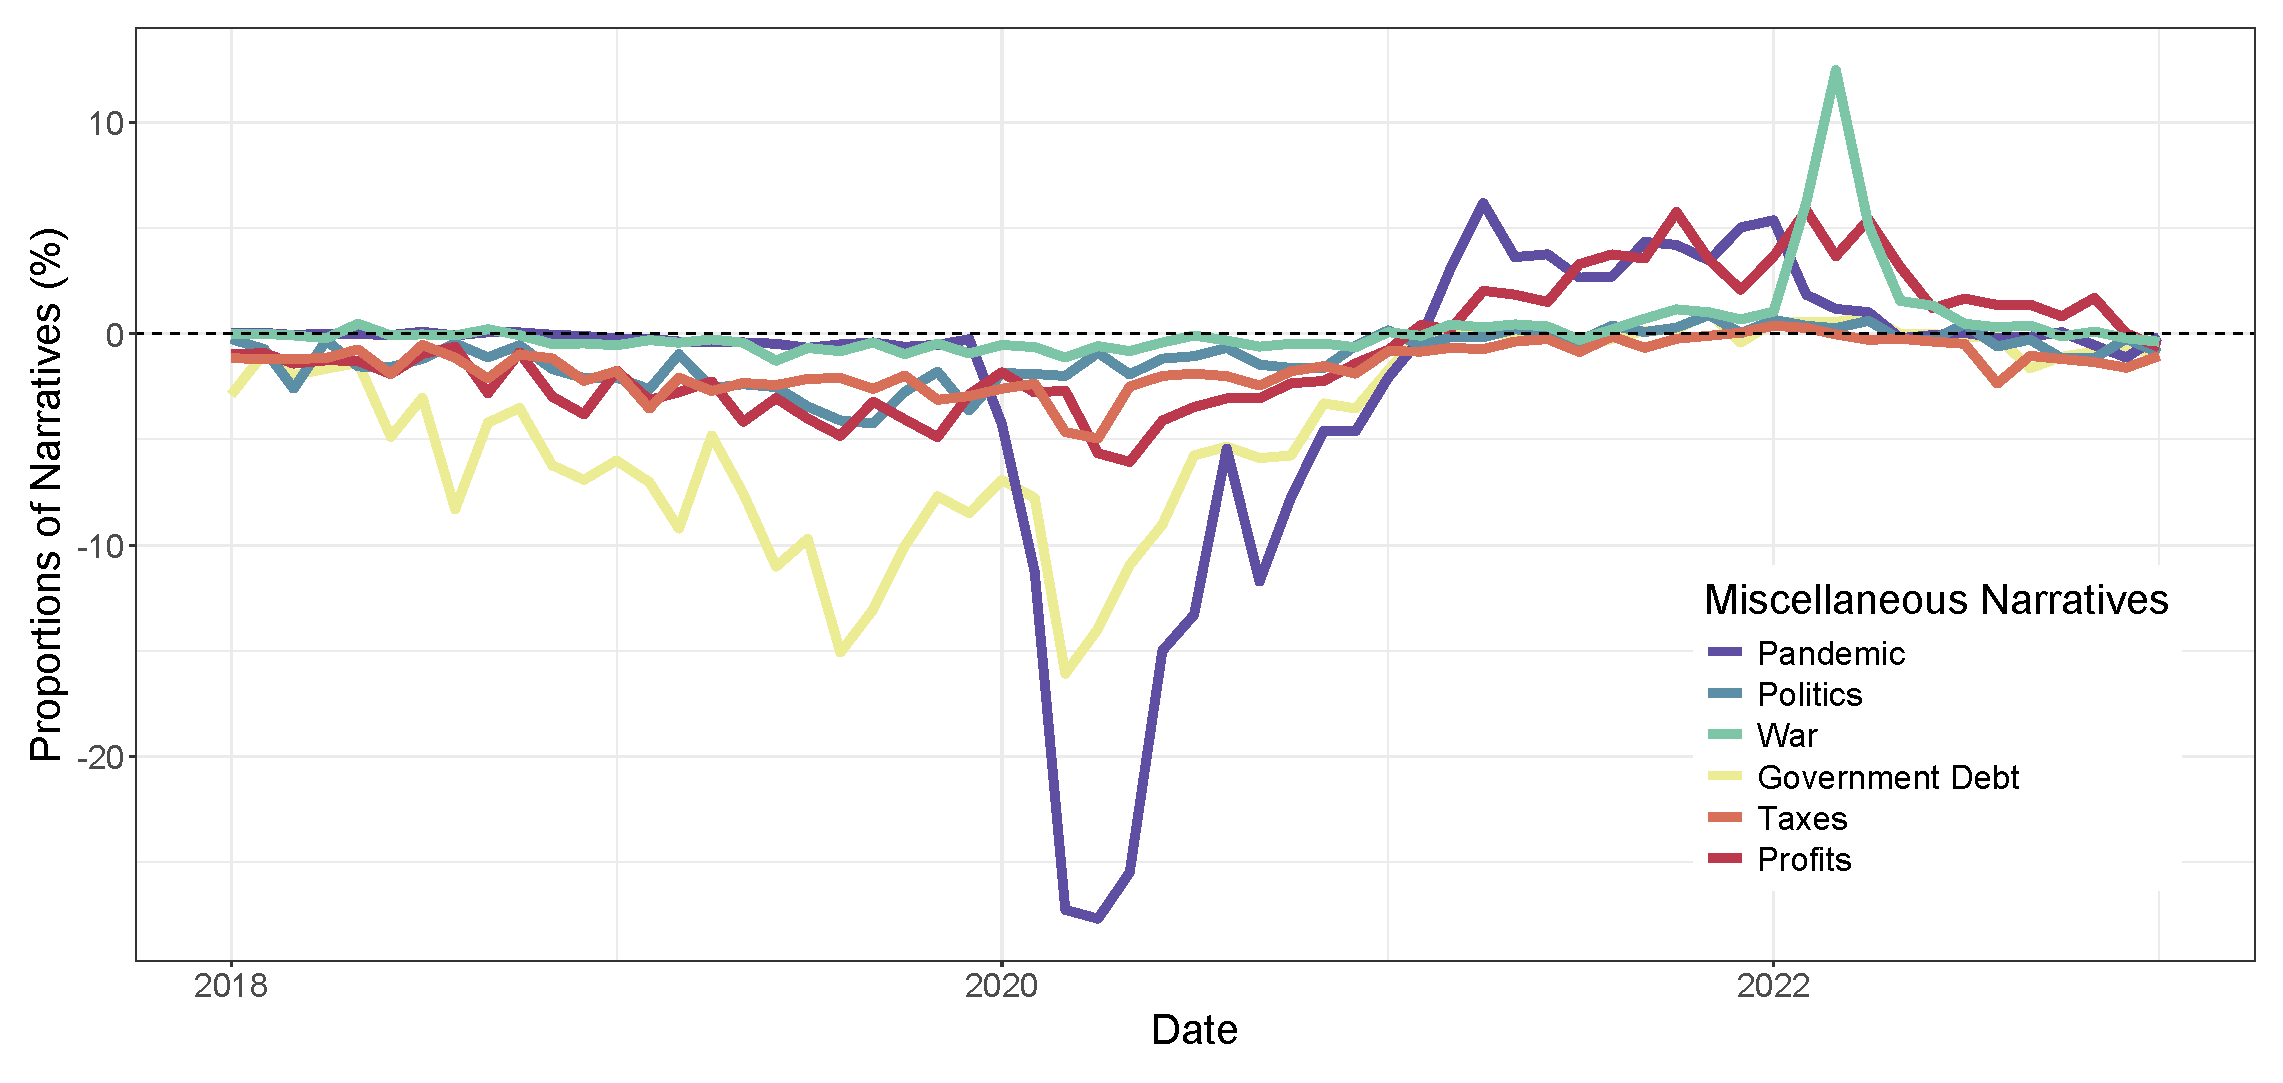
\includegraphics[width=\textwidth]{figures/plot_sothers.eps}
		\caption{Indices of miscellaneous narratives}
		\label{fig:sothers}
	\end{subfigure}
		\floatfoot{Note: The figures show the constructed narrative time series. Negative values signify the relative importance of a narrative in the context of falling inflation rates, whereas positive values represent the relative importance in the context of rising inflation rates.} 
\end{figure}

In contrast, the pent-up demand narrative reaches its minimum in early 2020, during the first announced economic lockdown following the COVID-19 outbreak. However, only a few months later, the narrative experiences significant positive growth. By 2021, it reaches relatively high positive values. The demand shift narrative also contributes to the media discourse about rising inflation rates but peaks with a lag compared to the pent-up demand narrative. Media reports on government spending as cause of inflation was not widespread during this entire period. We report only minor growth in late 2020 and early 2021. During this time, there were controversial discussions about large-scale infrastructure programs, which were questioned by Republicans and centrist Democrats (e.g., Peterson, 2021). In conclusion, we report positive values for all demand narratives from the beginning of 2021, but we observe significant differences in volume and timing.

Turning to the supply narratives, a similar trend becomes evident, with less negative values during the non-inflationary period. As Figure \ref{fig:ssupply} shows, only the energy narrative reaches profound negative values. In contrast, all three narratives show significant positive growth in 2020 and reach positive values in early 2021. Overall, all three narratives follow a similar path, with the supply chain reporting the steepest increase, whereas the energy narrative is more volatile. Additionally, it is the first among supply narratives to experience negative values already in mid-2022. Only the labor shortage narrative reports a positive score until the end of the observation period.

Larger differences among the narratives do we report for the miscellaneous. As figure \ref{fig:sothers} shows, the tax and politics narratives experience only minor changes, however, there is a slight increase from the end of 2020 to early 2021 for the politics narrative. In contrast, the pandemic narrative records pronounced changes and is highly polarized. While non existing until end of 2019, it experienced a remarkable decline during early 2020. This is in line with the spread of the COVID-19 virus and the associated non-pharmaceutical measures. However, the pandemic narrative is also rapidly recovers, besides a smaller setback in late 2020. The debt narrative is primarily experiencing a profound negative score in 2020, while it remained more or less insignificant during the inflationary period. Characterized by fewer extremes, the profit narrative is present in both periods. Further, the narrative is more persistent during the inflationary period with a comparably late peak in 2022. Lastly, the war narrative is not existing until early 2022, which coincides with the invasion of Russia in the Ukraine. It rapidly declines afterwards.


\subsection{Granger Causality}

So far, our analysis has revealed two key findings. First, combining survey study results with a semi-supervised topic model and a latent sentiment scaling technique enables us to measure and quantify known concepts of inflation narratives. Thus we are able to describe their evolution over time and identify narrative-specific polarity. Second, we provide descriptive evidence on the spread of inflation narratives. For the considered time period, those emphasizing changes in demand and its
strong recovery, monetary policy, and supply issues as causes of inflation are particularly notable. Additionally, our descriptive analysis has shown that narratives on profits and specific crisis-related aspects, such as pandemic or war in Ukraine, are highly featured in news media articles. In contrast, other narratives, including those on government spending, politics, debt, and taxes, are less often featured in reports about rising inflation rates.
	
To deepen our understanding of how inflation narratives interact with the macroeconomy, especially inflation expectations, we first construct multiple multivariate VAR models to test for potential Granger causalities in our system. The VAR models include short-term and mid-term expectations, CPI inflation, economic activity and one of the measured narrative indices. Even tough the procedure is based on predictability, and not on direct causal effects, we follow Granger's argument that predictive power can serve as an indicator for potential causalities \citep{shojaie.2022}. Additionally, by applying the test procedure in a more restrictive VAR setting we control relevant information beyond a bivariate relationship. In a second step we take existing economic research into account that indicates strong variations of inflation expectations among different socioeconomic groups (e.g., \citet{ecb.2021, Weber.etal.2022}). Further, pioneer survey studies suggest that the narratives of households are diverse and systematically related to individual characteristics (e.g., \citet{Andre.2023, Demgensky.2023}). To address this variation, we analyze disaggregated household expectations based on income, education, age, and numeracy, employing data from the New York Fed Survey of Consumer Expectations. Afterwards, we re-estimate our multivariate Granger causality tests by incorporating the expectations of subgroups (e.g. low income or high educated households) from each socioeconomic category to identify any potential Granger causal relationships.

\subsubsection{Aggregated Expectations}

As discussed in Chapter \ref{sec:MethodsData}, we treat all variables as trend-cycle filtered series and use them as baseline estimates. For robustness, we provide level and difference estimations in the Online Appendix. The results of the baseline estimation are shown in table \ref{tab:granger}. It provides a comprehensive overview of all p-values of the Granger causality analysis, indicating whether or not a narrative is Granger-causing 1-year or 3-year expectations. Thus, we test whether the integration of a narrative lag into a system of lagged variables improves the prediction of the households' expectations. As the table shows, we report several significant Granger-causal relationships.

For the demand narratives, we report significant results exclusively for the demand shift narrative at the aggregate level. For short-term expectations, we identify Granger-causal relationships for the supply chain and labor shortage narratives. For medium-term expectations, we confirm these results, but only for the supply chain narrative. Further Granger causalities are evident for the miscellaneous narratives, in this case for both expectations. This includes the war and profits narratives for short- and medium-term expectations. In summary, we find several highly significant Granger causalities for the narratives considered, with only minor changes between 1-year and 3-year expectations. In addition, we examine potential feedback relationships in table \ref{tab:granger_feedback}. We test the exogeneity of the narratives with respect to aggregate expectations. Among the previous Granger causalities, our estimation suggests a feedback relationship with 3-year expectations only for the supply chain narrative. We also find some reverse Granger causality for the pent-up demand and energy narratives from 1-year expectations and for energy from 3-year expectations. 

\begin{table}[ht]
\centering
\caption{Narrative $\rightarrow$ Expectations Granger causality (boosted HP-Filter)}\label{tab:granger}

\begin{tabular}{lcc}
\toprule
\textbf{Narratives} & \textbf{One-Year Expectations} & \textbf{Three-Year Expectations} \\
& (Pr($>$F)) & (Pr($>$F)) \\
\midrule
\multicolumn{3}{l}{\textbf{Demand}} \\
\midrule
Government Spending & 0.29 & 0.09 * \\
Monetary Policy & 0.64 & 0.23 \\
Demand Shift & 0.16 & 0.41 \\
Demand (residual) & 0.80 & 0.96 \\
\midrule
\multicolumn{3}{l}{\textbf{Supply}} \\
\midrule
Supply Chain & $<$0.01 *** & 0.10 * \\
Energy & 0.75 & 0.34 \\
Labor Shortage & $<$0.01 *** & 0.38 \\
Supply (residual) & 0.52 & 0.39 \\
\midrule
\multicolumn{3}{l}{\textbf{Miscellaneous}} \\
\midrule
Pandemic & 0.39 & 0.23 \\
Politics & 0.57 & 0.95 \\
War & 0.04 ** & 0.04 ** \\
Debt & 0.11 & 0.86 \\
Taxes & 0.91 & 0.29 \\
Profits & 0.02 ** & $<$0.01 *** \\
\midrule
\bottomrule
\textit{Note:}  & \multicolumn{2}{r}{$^{*}$p$<$0.1; $^{**}$p$<$0.05; $^{***}$p$<$0.01} \\
\bottomrule
\end{tabular}
\end{table}


To ensure robustness, we provide additional level and difference estimations in the Online Appendix in tables \ref{tab:granger_level} and \ref{tab:granger_diff}. Overall, the results with the boosted HP filter are confirmed by the level estimates, although more significant relationships are reported. In contrast to the trend-cycle filtered estimation, these results suggest Granger causality for monetary policy, labor shortage, and politics on 3-year expectations. The results are supported for the demand shift, supply chain, labor shortage (1-year expectations), and profit narrative for short- and/or medium-term expectations. In comparison, the difference estimations give a more restrictive picture, but all of the Granger causalities for short-term expectations are supported. In contrast, for medium-term expectations, the estimation only supports the initial results for the demand shift. In addition, we report significant results for the government spending narrative. 

At last,  our results suggest that narratives featured in media reports possess inherent statistical predictive power for household expectations. This can be interpreted as an indicator of potential causalities \cite{shojaie.2022}. Moreover, our findings suggest that Granger causalities are present in all categories, but there are slight differences in the data between short-term and medium-term expectations.  To address the challenge of potential nonstationarity, we consider results with three different estimation strategies. Although we find some differences between these estimations, most of the results, especially for short-term expectations, are confirmed. Moreover, correlative evidence from \cite{Andre.2023} and \cite{Stantcheva.2024} backs our findings regarding how important supply and profit narratives are for 1-year expectations. In contrast to these survey studies, we do not report significant p-values for the politics, monetary policy, and government spending narratives on aggregate expectations. This could be partly explained by the considered news source, which targets financial market actors and experts. 

\begin{table}[ht]
\centering
\caption{Expectations $\rightarrow$ Narrative Granger causality (boosted HP-Filter)}\label{tab:granger_bHP_feedback}

\begin{tabular}{lcc}
\toprule
\textbf{Narratives} & \textbf{One-Year Expectations} & \textbf{Three-Year Expectations} \\
& (Pr($>$F)) & (Pr($>$F)) \\
\midrule
\multicolumn{3}{l}{\textbf{Demand}} \\
\midrule
Government Spending & 0.56 & 0.85 \\
Monetary Policy & 0.64 & 0.54 \\
Demand Shift & 0.78 & 0.59 \\
Demand (residual) & $<$0.01 *** & 0.32 \\
\midrule
\multicolumn{3}{l}{\textbf{Supply}} \\
\midrule
Supply Chain & 0.16 & 0.20 \\
Energy & 0.05 * & 0.02 ** \\
Labor Shortage & 0.42 & 0.04 ** \\
Supply (residual) & 0.04 ** & 0.53 \\
\midrule
\multicolumn{3}{l}{\textbf{Miscellaneous}} \\
\midrule
Pandemic & 0.12 & 0.30 \\
Politics & 0.89 & 0.97 \\
War & 0.93 & 0.75 \\
Debt & 0.41 & 0.89 \\
Taxes & 0.50 & 0.88 \\
Profits & 0.73 & 0.73 \\
\midrule
\bottomrule
\textit{Note:}  & \multicolumn{2}{r}{$^{*}$p$<$0.1; $^{**}$p$<$0.05; $^{***}$p$<$0.01} \\
\bottomrule
\end{tabular}
\end{table}


\subsubsection{Socioeconomic Heterogeneity}

\textbf{Heterogeneity by Income} - We begin the discussion of socioeconomic heterogeneity by looking at differences in income. The New York Fed survey distinguishes three income groups: below \$50k, \$50k to \$100k, and above \$100k per year. The results in table \ref{tab:granger_income} in the Online Appendix show some differences between the considered groups. With respect to short-term expectations, our results suggest only small distinctions between the different income groups. What is significant for all groups are the demand shift, supply chain, labor shortage, and profit narratives. However, for the lower- and middle-income groups, we additionally report significant results for the war narrative. We report significant results for the pandemic narrative solely for middle- and upper-income households. In contrast, we observe stronger heterogeneity across incomes for medium-term expectations. Our results emphasize the significance of demand narratives for middle- and high-income households, while significant effects appear only for the energy narrative among lower-income households. Our analysis suggests that the 3-year expectations of middle-income households appear to respond only to demand narratives. In contrast, we report multiple Granger causal relationships for high income-households, including narratives demand, supply, and miscellaneous narratives.\\


\noindent \textbf{Heterogeneity by Education} - To access further potential heterogeneity of narratives across socioeconomic groups, we conduct Granger tests for different educational backgrounds of households. Accordingly, we consider the household groups with a high school degree or less, some college, and a BA or higher. The results are shown in table \ref{tab:granger_educ} in the Online Appendix. As our analysis suggests, households with high levels of education are more responsive to narratives that emphasize demand shifts, supply chain issues, or profits. However, we find partly similar results for all household groups. The pandemic and war narratives are also important for high educated households' medium-term expectations. In contrast, we observe significant results for households with some college education or less with regard to government spending. Interestingly, this is the only Granger causality to 3-year expectations we observe for this group. Lastly, the data suggest that the labor shortage narrative Granger-causes short-term expectations of households with some college degree or less.\\

\noindent \textbf{Heterogeneity by Age} - Pronounced variations with respect to age are visible in \ref{tab:granger_age} in the Online Appendix. As before, we observe less heterogeneity across different ages for short-term expectations than for medium-term expectations. For the analysis, we consider three groups: under 40, 40 to 59, and over 59. Overall, we find fewer Granger causality relationships for the oldest households. Moreover, for households aged 40 and older, demand narratives are significant. Further, for these households numerous supply narratives are particularly important for short-term expectations. In contrast, we observe the most Granger-causal relationships for miscellaneous narratives among the youngest cohort. Overall, this analysis highlights the relevance of age as a determinant of heterogeneity across households. \\

\noindent\textbf{Heterogeneity by Numeracy} - Finally, we examine potential heterogeneity between households with low and high numeracy in table \ref{tab:granger_num} in the Online Appendix. Overall, our analysis indicates only minor differences for 3-year expectations. Comparatively, our results indicate strong differences among households' short-term expectations. For households with a lower numeracy, our analysis highlights the importance of the war and pandemic narratives. For high numeracy households, more Granger-causal relationships for the supply and demand narratives are present. Furthermore, we again identify that the profit narrative is relevant for short-term expectations.

\subsubsection{Dynamic Responses}

To further investigate potential causal relationships between our narratives and households' expectations, we estimate impulse responses. This approach allows us to gain a more comprehensive understanding of the impact that an increasing diffusion of narratives has at the macroeconomic level. In the following section, we provide an overview of the impulse responses that we conducted by means of \cite{Jorda.2005}'s local projections. In this process, the impulse responses measure the effect of an impulse to the system, i.e. how an impulse at a specific point of time $t_0$ in one equation proceeds through a system \citep[138]{Kirchgaesser.2007}. In this case, we consider a shock the size of one standard deviation of the error term. We conduct several multivariate models that contain five different variables: 1-year and 3-year expected inflation by households, CPI inflation, economic activity, and one of our constructed narrative indices. Again, as mentioned in chapter \ref{subsec:methods}, we treat all variables as trend-cycle filtered time series and use them as a baseline. For the robustness, we estimated the local projections with levels and differences. To ensure readability and an efficient use of the limited space, we included all graphical illustrations of the impulse responses in the Online Appendix. The complete set of baseline impulse responses are illustrated in figure \ref{fig:irf_1}, \ref{fig:irf_2}, \ref{fig:irf_3}, and \ref{fig:irf_4} in the Online Appendix. Figure \ref{fig:irf_base} reports a selection of significant responses. The x-axis represents the forecast horizon $s$, with a maximum of 12 months, while the y-axis shows the change in 1- or 3-year household expectations in response to a standardized deviation innovation. The black line represents the mean response to a shock, while the gray area around the line visualizes the 90\% confidence interval.

We begin by examining the response to demand narrative shocks. In doing so, we observe statistically significant positive responses for all demand narratives. Comparatively, we note some differences in the paths of the responses. The shock in the government spending narrative is the longest lasting among the demand narratives. The response to a shock in the demand shift narrative is of the same magnitude but of shorter duration, while we also observe a smaller magnitude for the monetary policy narrative. Only initially positive reacts the medium-term expectations to a shock in the pent-up demand narrative. These findings are consistent with the positive coefficients for the monetary policy and government spending narratives in \cite{Andre.2023}. The impulse responses for the supply chain narrative are in line with the discussion about its anchoring tendency in \cite{Andre.2023, Demgensky.2023}. The response is short-lived and temporarily negative. While there is a primarily statistically significant reaction only for the energy narrative, the relevance of the supply chain and labor shortage narrative for household expectations is again highlighted. For the latter, the response is profound and comparatively persistent. Finally, the ways in which the miscellaneous narratives react to a shock are more diverse, with a large number of responses being insignificant. We establish only partially significant results for short-term expectations to a shock in the pandemic narrative, which are initially negative, before they turn positive over time. In contrast, a shock to the politics narrative seems to initially raise expectations, especially in the medium-term, and then return to the baseline. Furthermore, the war narrative and the profits narrative should be emphasized. The profits narrative indicates positive responses in both expectations, which are also relatively strong in terms of magnitude, with a rather transient effect on 3-year expectations. The response to the war narrative is exceptional considering its strong decreasing tendency after an initial increase. Overall, the results are roughly in line with our previous findings and the results of the survey conducted by \cite{Andre.2023, Stantcheva.2024, Demgensky.2023}. 


\begin{figure}[H]
	\centering
	\captionsetup{font=footnotesize}
	\begin{subfigure}{00.32\textwidth}
		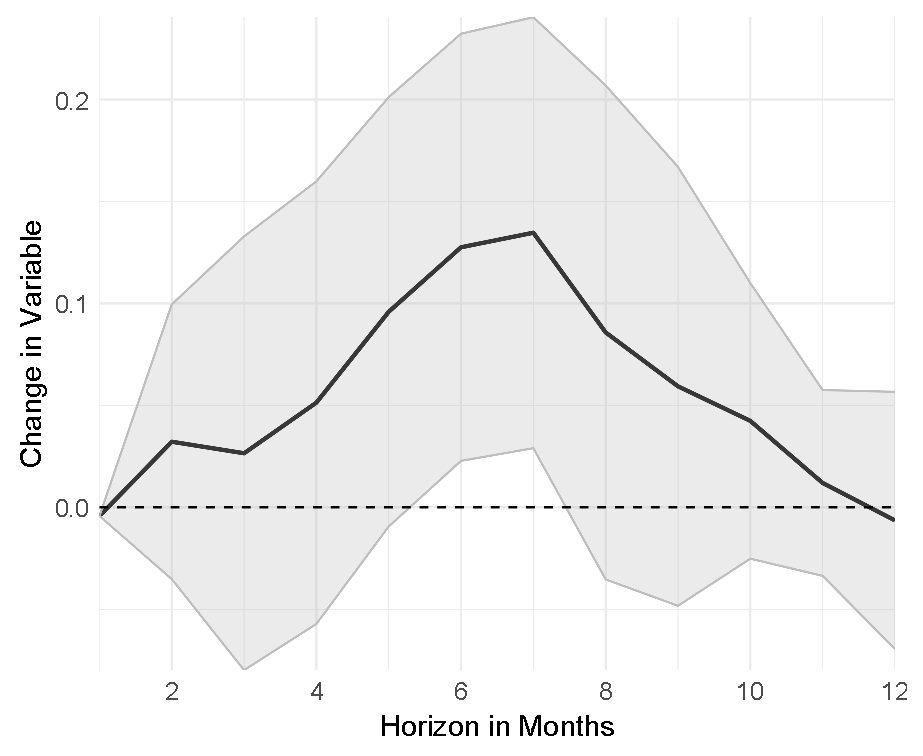
\includegraphics[width=1\textwidth]{output/lp/baseline/bHP/government_spending/government_spendingonexpectations1y_djn.eps}
		\caption{Government spending on 1-year}
	\end{subfigure}
	\begin{subfigure}{00.32\textwidth}
		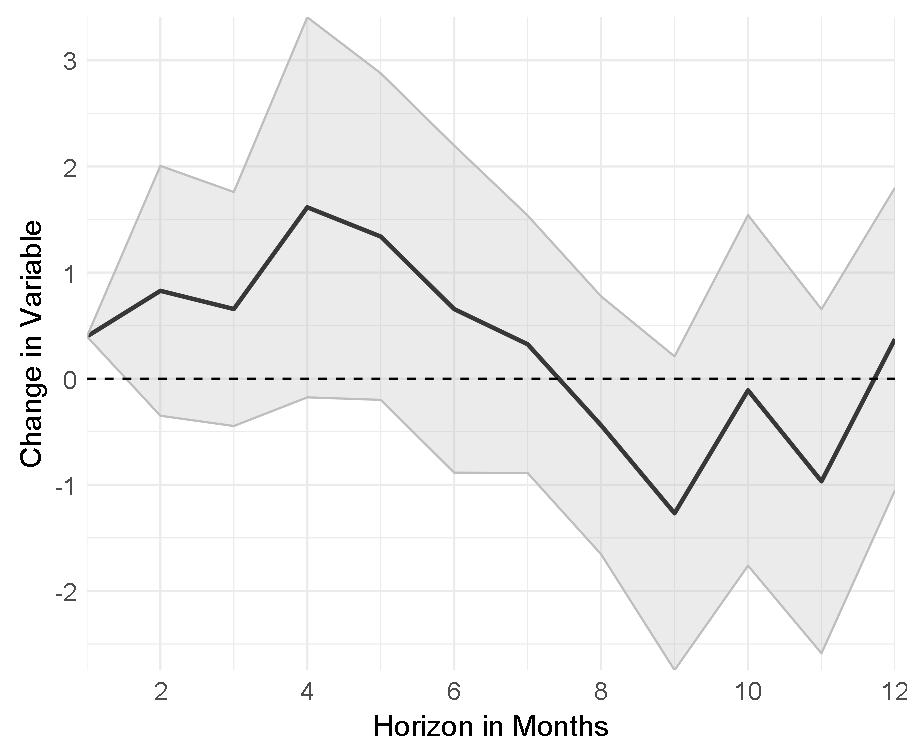
\includegraphics[width=1\textwidth]{output/lp/baseline/bHP/monetary_policy/monetary_policyonexpectations3y_djn.eps}
		\caption{Monetary policy on 3-year}
	\end{subfigure}
	\begin{subfigure}{00.32\textwidth}
		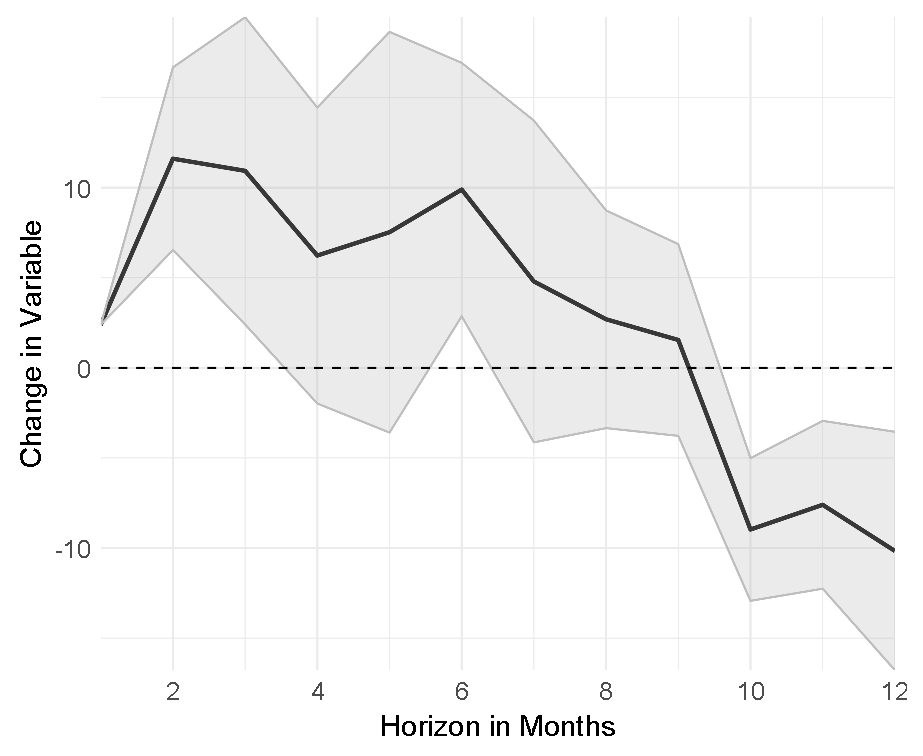
\includegraphics[width=1\textwidth]{output/lp/baseline/bHP/supply_chain/supply_chainonexpectations1y_djn.eps}
		\caption{Supply chain on 1-year}
	\end{subfigure}
	\begin{subfigure}{00.32\textwidth}
		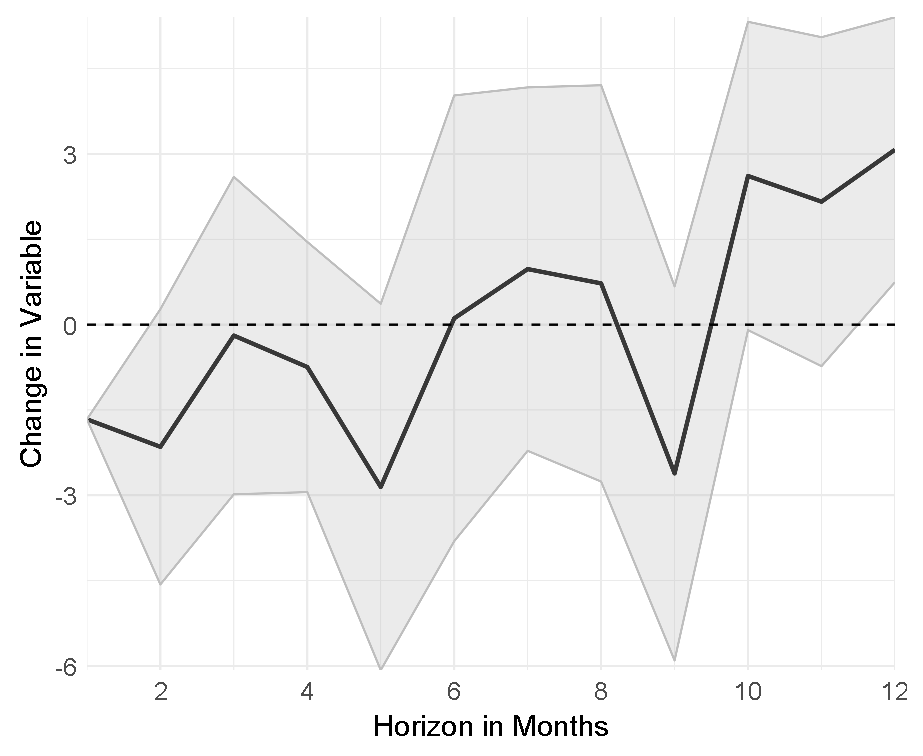
\includegraphics[width=1\textwidth]{output/lp/baseline/bHP/pandemic/pandemiconexpectations1y_djn.eps}
		\caption{Pandemic on 1-year}
	\end{subfigure}
	\begin{subfigure}{00.32\textwidth}
		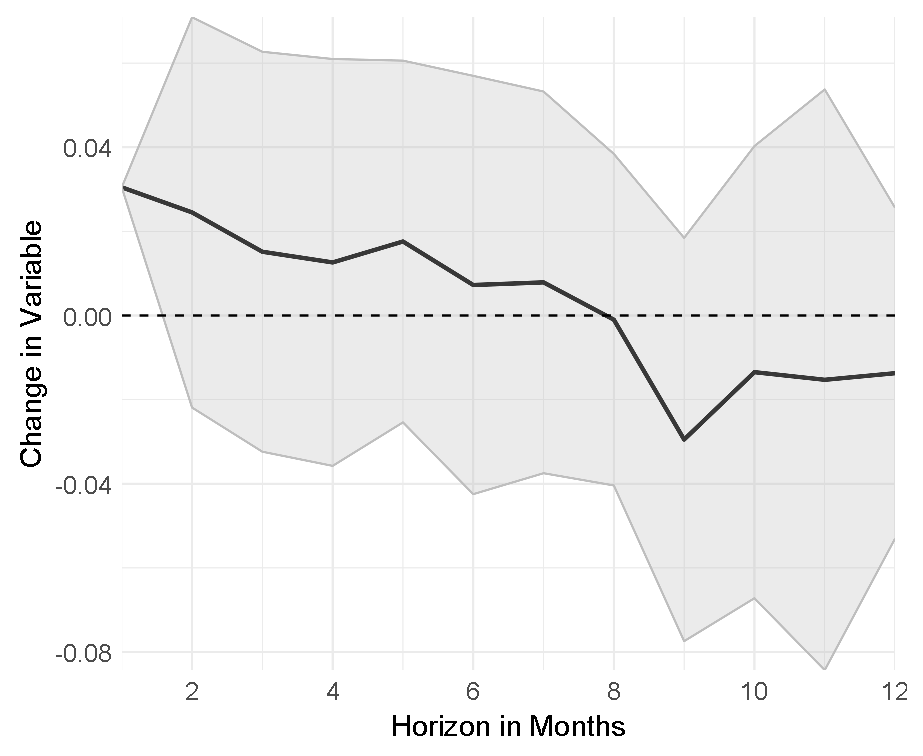
\includegraphics[width=1\textwidth]{output/lp/baseline/bHP/politics/politicsonexpectations3y_djn.eps}
		\caption{Politics on 3-year}
	\end{subfigure}
	\begin{subfigure}{00.32\textwidth}
		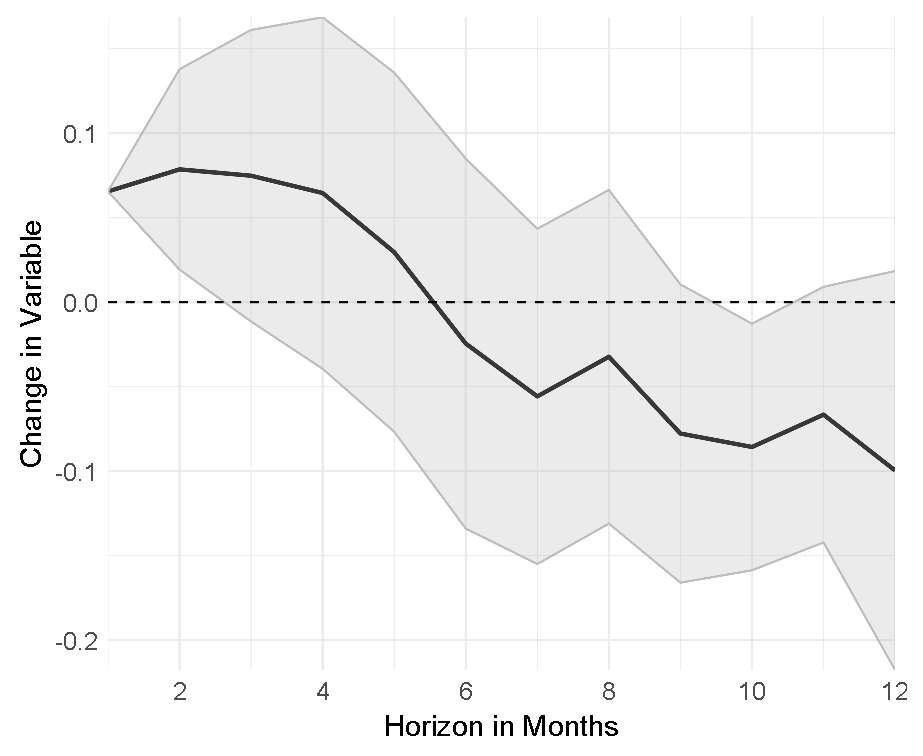
\includegraphics[width=1\textwidth]{output/lp/baseline/bHP/war/waronexpectations1y_djn.eps}
		\caption{War on 1-year}
	\end{subfigure}
	\begin{subfigure}{00.32\textwidth}
		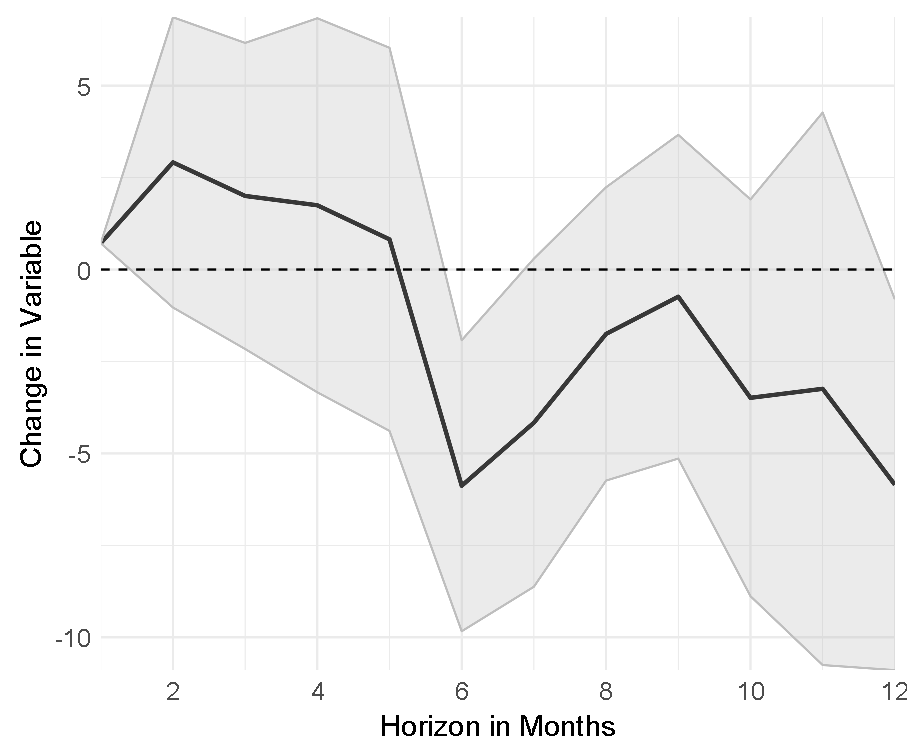
\includegraphics[width=1\textwidth]{output/lp/baseline/bHP/war/waronexpectations3y_djn.eps}
		\caption{War on 3-year}
	\end{subfigure}
	\begin{subfigure}{00.32\textwidth}
		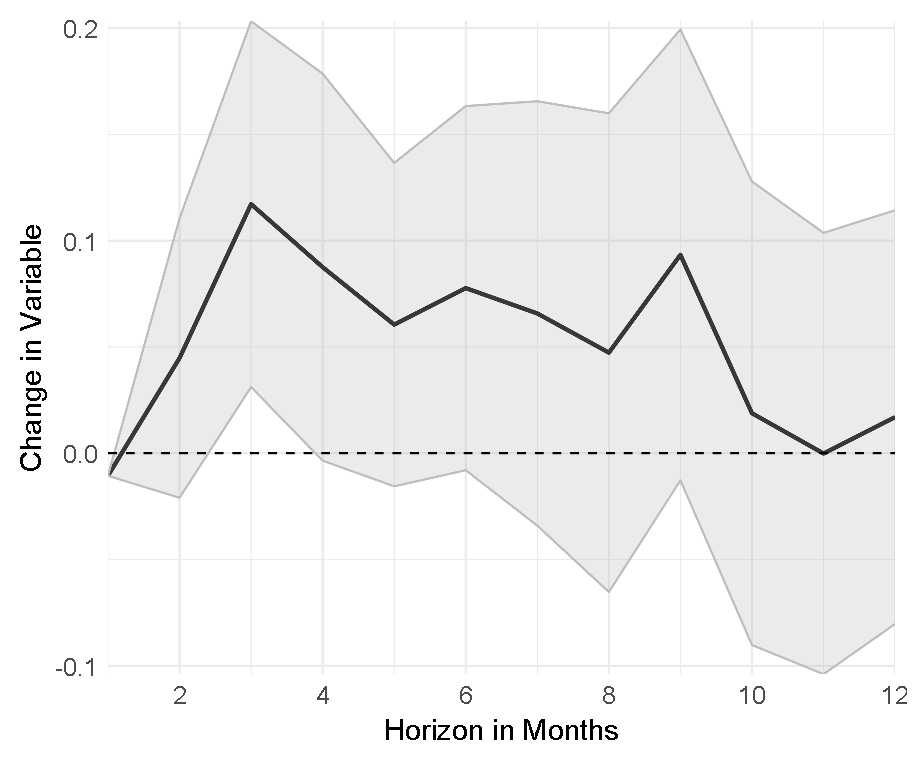
\includegraphics[width=1\textwidth]{output/lp/baseline/bHP/profits/profitsonexpectations1y_djn.eps}
		\caption{Profits on 1-year}
	\end{subfigure}
	\begin{subfigure}{00.32\textwidth}
		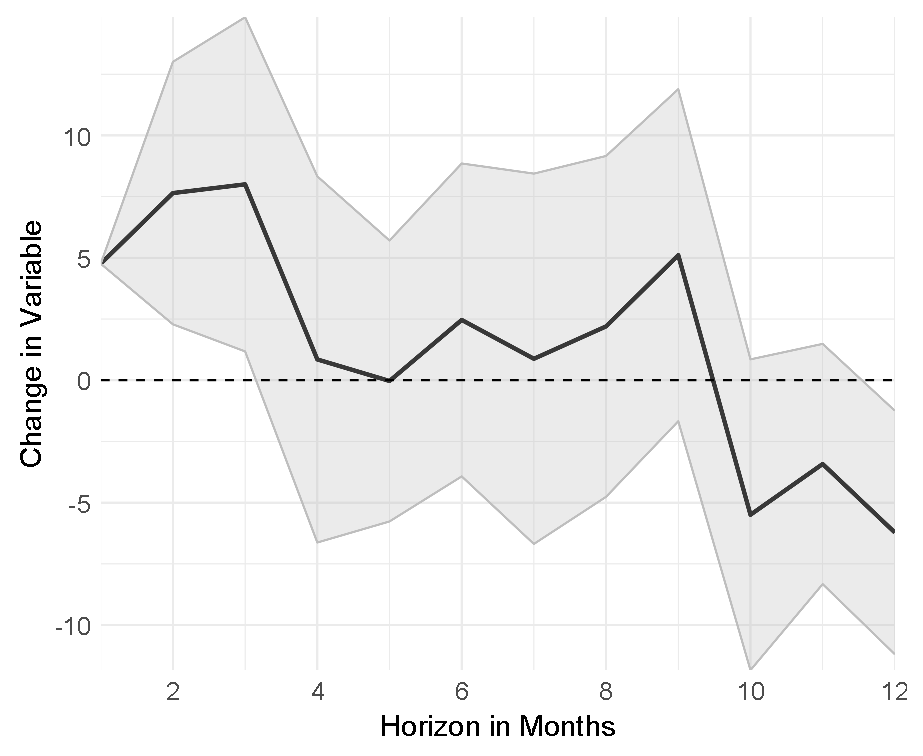
\includegraphics[width=1\textwidth]{output/lp/baseline/bHP/profits/profitsonexpectations3y_djn.eps}
		\caption{Profits on 3-year}
	\end{subfigure}
	\caption{Selection of narratives' impulse responses}
	\label{fig:irf_base}
	\floatfoot{Note: The graphs show the mean responses and 90\% confidence bands. The x-axis shows months (s) after narrative diffusion event; t = 0 is the month of the shock event. The y-axis shows the change in expectations as a response to the shock event. The shock considered is of the size of one standard deviation.}
\end{figure}



To summarize the analysis of aggregate expectations, it can be concluded that a (positive) narrative shock is followed by an initial positive response of households' expectations. At the same time, a closer look reveals differences in the paths of the responses. Comparing 1-year and 3-year expectations, the response in 1-year expectations is more pronounced in terms of magnitude and, in many cases, more persistent. The results also highlight some important differences between the narratives. While our results indicate significant positive responses for most demand and supply narratives, the responses of the latter are less persistent and in some cases insignificant for 3-year expectations, suggesting a stronger anchoring tendency of these narratives. On the other hand, the responses to a shock in the other narratives are more diverse. Among these, the profit narrative stands out for its profound effect on short-term expectations.

As for the Granger causality tests, we provide robustness estimates again using levels and differences. The results for the selected impulse responses from figure \ref{fig:irf_base} are shown in the Online Appendix with level specification in figure \ref{fig:irf_level}, and figure \ref{fig:irf_diff} visualized the results with the differences. While the responses under level specification are more persistent, the responses with differences time series are more ambivalent and unstable. In general, the robustness estimations support our findings. However, for the pandemic narrative only, both robustness estimations indicate no significant reaction in household expectations. It should be noted, that the baseline estimation indicates an overall stronger anchoring tendency of expectations.
